% !TeX spellcheck = cs_CZ
%{\tikzset{external/prefix={tikz/FYZI/}}
% \tikzset{external/figure name/.add={ch31_}{}}
%=========================== Kapitola: Původ indexu lomu ==========================================
\setchaptertoc
\chapter{Původ indexu lomu}\label{fyz:IchapXXXI}

  \section{Index lomu}\label{fyz:IchapXXXIsecI}
  \section{Pole v látce}\label{fyz:IchapXXXIsecII}
    \begin{equation}\label{fyz:eq966}
      E_s=E_0\exp{\imath\omega(t-z/c)}.
      \end{equation}
  \section{Disperze}\label{fyz:IchapXXXIsecIII}
  \section{Absorpce}\label{fyz:IchapXXXIsecIV}
  \section{Energie přenášená elektrickou vlnou}\label{fyz:IchapXXXIsecV}
  \section{Difrakce světla na cloně}\label{fyz:IchapXXXIsecVI}
  \section{Příklady a cvičení}\label{fyz:IchapXXXIsecVII}

    \begin{figure}[ht!] %\ref{fyz:fig0261}
      \centering
      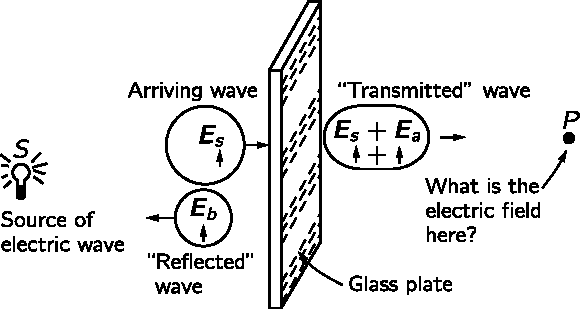
\includegraphics[width=0.9\linewidth]{fyz_fig0261.pdf}
      \caption{Elektromagnetická vlna při průchodu vrstvou průhledné látky
               (\cite[s.~411]{Feynman01})}
      \label{fyz:fig0261}
    \end{figure}

    \begin{figure}[ht!] %\ref{fyz:fig0262}
      \centering
      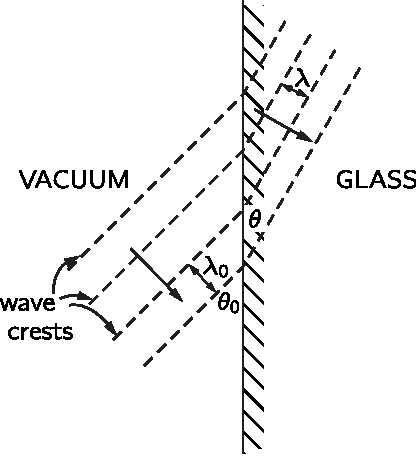
\includegraphics[width=0.9\linewidth]{fyz_fig0262.pdf}
      \caption{Vztah mezi lomem vln a změnou jejich rychlosti
               (\cite[s.~412]{Feynman01})}
      \label{fyz:fig0262}
    \end{figure}

    \begin{figure}[ht!] %\ref{fyz:fig0263}
      \centering
      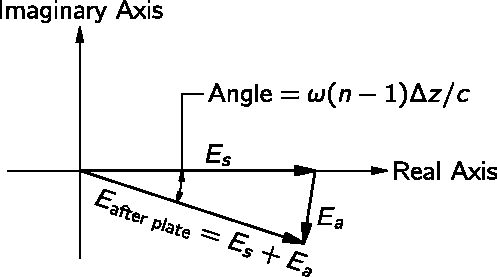
\includegraphics[width=0.9\linewidth]{fyz_fig0263.pdf}
      \caption{Graf k určení prošlé vlny pro dané \(t\) a \(z\)
               (\cite[s.~413]{Feynman01})}
      \label{fyz:fig0263}
    \end{figure}
    
    \begin{figure}[ht!] %\ref{fyz:fig0264}
      \centering
      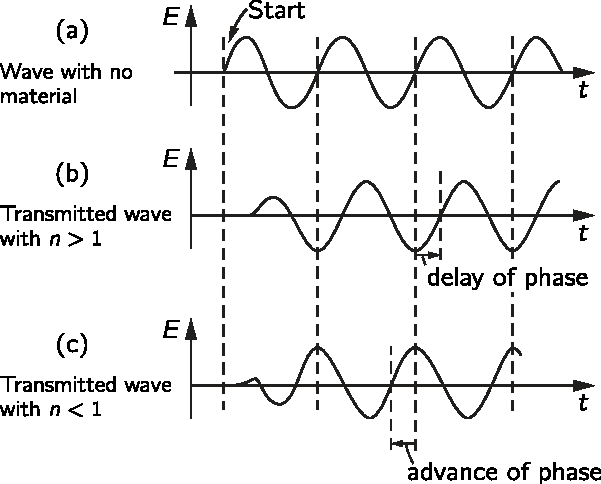
\includegraphics[width=0.9\linewidth]{fyz_fig0264.pdf}
      \caption{Vlnové signály
               (\cite[s.~418]{Feynman01})}
      \label{fyz:fig0264}
    \end{figure}

    \begin{figure}[ht!] %\ref{fyz:fig0265}
      \centering
      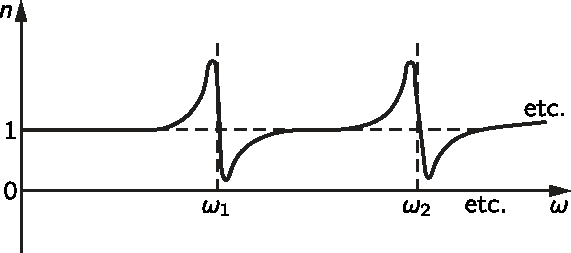
\includegraphics[width=0.9\linewidth]{fyz_fig0265.pdf}
      \caption{Index lomu jako funkce frekvence
               (\cite[s.~419]{Feynman01})}
      \label{fyz:fig0265}
    \end{figure}
    

    \begin{figure}[ht!]  %\ref{fyz:fig0266}
      \centering
      \subcaptionbox{\label{fyz:fig0266a}}{\luafigure[0.8]{fyz_fig0266a.pdf}}               \\
      \subcaptionbox{\label{fyz:fig0266b}}{\luafigure[0.8]{fyz_fig0266b.pdf}}               \\
      \subcaptionbox{\label{fyz:fig0266c}}{\luafigure[0.8]{fyz_fig0266c.pdf}}
      \caption{Difrakce na stínítku
               (\cite[s.~422]{Feynman01})}
      \label{fyz:fig0266}
    \end{figure}

%} %tikzset
%---------------------------------------------------------------------------------------------------